\documentclass[11pt]{article}
\usepackage[margin=2cm]{geometry}
\usepackage{graphicx}
\usepackage{titling} %For document header
\usepackage{apacite}
\usepackage{float}

\begin{document}
\begin{titlepage}
	
\includegraphics[height = 35mm, width = 32mm]{../Writeup/crest.png}%
	\hfill
	
\includegraphics[height = 30mm, width = 90mm]{../Writeup/zsl.png}
	
		\centering
		
		\vspace{5cm}
		%Thesis title
		{\uppercase{\textbf{\LARGE Application of Random Encounter Model to Estimate Population Densities Using Unmanned Aerial Vehicles \\}}}
		\vspace{6cm}
		%Author's name
		\begin{minipage}[t]{0.4\textwidth}
			\begin{flushleft} \large
				\emph{Author:} \\
				Eva Linehan\\
				e.linehan18@imperial.ac.uk
			\end{flushleft}
		\end{minipage}
		\begin{minipage}[t]{0.4\textwidth}
			\begin{flushright} \large
				\emph{Supervisor:} \\
				Dr. Marcus Rowcliffe \\
				Dr. Tom Letessier
			\end{flushright}
		\end{minipage}\\[3cm]
		
		Computational Methods in Ecology and Evolution\\
		Imperial College London\\
		April 2019\\
	%\end{center}
\end{titlepage}



\section{Keywords}
population monitoring, UAV, REM, encounter rate, gREM, absolute animal density

\section{Introduction}
Monitoring animal populations has never been more important with rapid habitat and climatic changes resulting from increased anthropogenic activity (). Sensor technologies are becoming progressively more widespread in order to monitor population density and abundance. In marine and coastal environments, unmanned aerial vehicles (UAVs) have been successful in documenting the spatio-temporal dynamics of large faunal assemblages \cite{colefax2019reliability}. However, estimating marine wildlife densities or abundance often requires individual recognition of animals (photo identification, capture-mark-recapture methods) or knowing the distance of the animal from the sensor (distance sampling), which is often difficult \cite{Lucas}. The random encounter model (REM), developed from the classical ideal gas model, enables animal densities to be estimated given the velocity of both the animal and sensor (if mobile), as well as other sensor parameters \cite{rowcliffe}. The original ideal gas model was used in physics to predict the collision rate of molecules given molecule density, mean speed and size. Following multiple biological applications to predict the encounter rate of moving animals, the encounter-rate equation was reversed to estimate the density of target species encountered during surveys \cite{yapp1956theory}. Limitations, including confidence intervals for expected encounter rates and the absolute random movement of individuals, can be accounted for through slight modification of this equation \cite{hutchinson2007use}. This simplified model can be used in two or three dimensions to estimate encounter rates of a target species but despite it's flexibility, it has not been widely reported in the literature. The aim of this study is to develop a generalized random encounter model (gREM) to estimate absolute animal density from count data in the marine environment. Parameters from the model will be derived from UAV data (speed distribution, home ranges, overlaps, area monitored) as well as known environmental factors (water visibility).  

\section{Methods}
Rate of contact of marine wildlife (dolphins, crocodiles, manatees, seabirds, sharks) will be derived from georeferenced images, stemming from fixed-wing UAV surveys in the Turneffe Marine Reserve (Belize) and off the coast of New Caledonia (French Polynesian Islands). The gREM will be based on that of Lucas \textit{et al.,} 2015, but modified to the marine environment whilst accounting for a moving sensor. Model modifications will be made according to those outlined by Hutchinson \& Waver, 2007. The accuracy and precision of the model will be investigated using Monte Carlo simulations of different combinations of sensor parameters. Sensor parameters include camera width, UAV altitude, flight speed, and proportion of time spent at the surface by the animal, as reported in previous studies. 



\section{Anticipated Outcomes}
The overall objective of this project is to create a generalized Random Encounter Model to accurately assess absolute animal densities in marine protected areas using UAVs. This will provide an expected baseline for population density estimates in specific marine protected areas that can reviewed with more data. As the role of UAVs in population monitoring increases, this method can be applied across different datasets to improve conservation efforts.


\section{Project Feasibility}

\begin{figure}[H]
	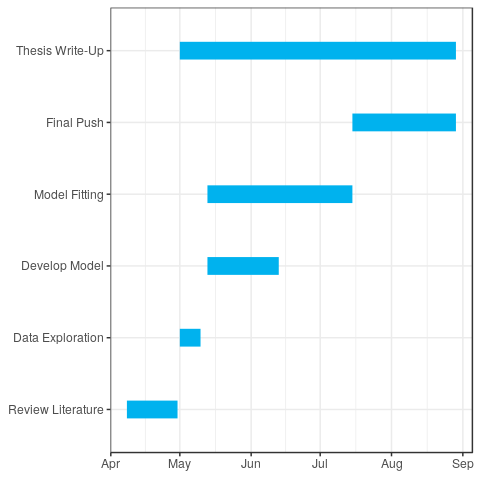
\includegraphics[height = 12cm, width=14cm]{../Data/gantt.png}
	\caption{Gantt chart outlining the proposed timeline from April 2019 to September 2019. This includes 1) preliminary literature review; 2) exploration of the original dataset; 3) gREM model development; 4) Model fitting and re-fitting to extended dataset ; 5) final push; and 6) thesis writing.}
\end{figure}

\section{Budget}
The entirety of the project budget (£500) will be allocated to travelling to ZSL in order to avail of the desk space provided. This is necessary for ongoing close collaboration with both supervisors.
The cheapest return ticket is priced at £12 which will allow for 2 journeys a week.

\bibliographystyle{apacite}
\bibliography{../Writeup/References.bib}


%\college{Imperial College London}


\end{document}